\documentclass[border=15pt]{standalone}
\usepackage{amsmath, amssymb}
\usepackage{tikz}
\usetikzlibrary{arrows.meta}

\definecolor{block0}{HTML}{E53935}
\definecolor{block1}{HTML}{1E88E5}
\definecolor{block2}{HTML}{43A047}
\definecolor{block3}{HTML}{FB8C00}
\definecolor{block4}{HTML}{8E24AA}

\begin{document}
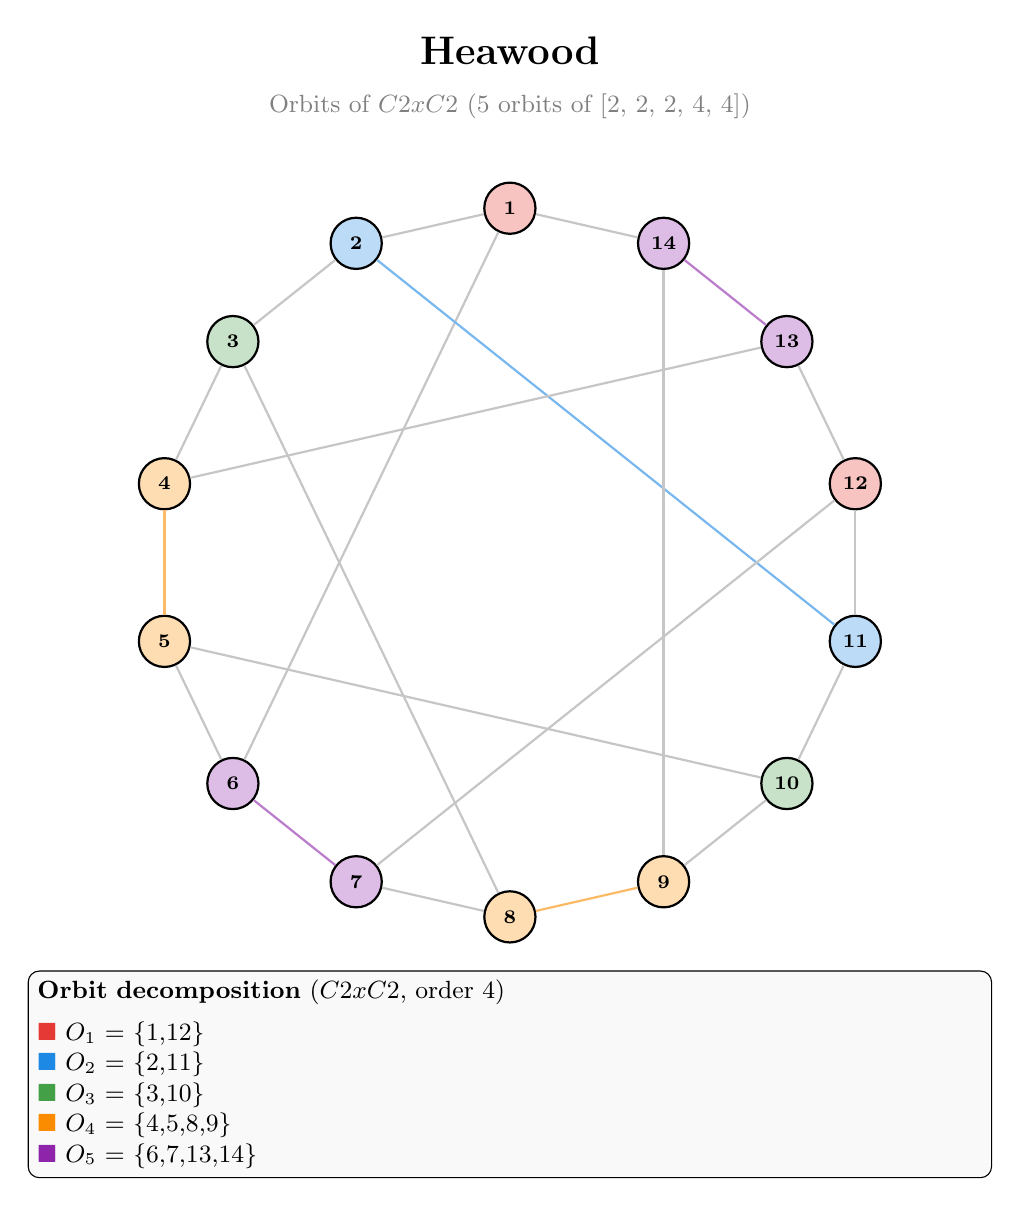
\begin{tikzpicture}[
  vertex/.style={circle, draw, thick, minimum size=6.5mm, inner sep=0pt,
                 font=\scriptsize\bfseries},
  edge/.style={thick, gray!45},
  title/.style={font=\Large\bfseries},
  subtitle/.style={font=\small, text=gray},
]

\node[title] at (0, 6.5) {Heawood};
\node[subtitle] at (0, 5.8) {Orbits of $C2 x C2$ (5 orbits of [2, 2, 2, 4, 4])};

\node[vertex, fill=block0!30] (v1) at (0.000, 4.500) {1};
\node[vertex, fill=block1!30] (v2) at (-1.952, 4.054) {2};
\node[vertex, fill=block2!30] (v3) at (-3.518, 2.806) {3};
\node[vertex, fill=block3!30] (v4) at (-4.387, 1.001) {4};
\node[vertex, fill=block3!30] (v5) at (-4.387, -1.001) {5};
\node[vertex, fill=block4!30] (v6) at (-3.518, -2.806) {6};
\node[vertex, fill=block4!30] (v7) at (-1.952, -4.054) {7};
\node[vertex, fill=block3!30] (v8) at (-0.000, -4.500) {8};
\node[vertex, fill=block3!30] (v9) at (1.952, -4.054) {9};
\node[vertex, fill=block2!30] (v10) at (3.518, -2.806) {10};
\node[vertex, fill=block1!30] (v11) at (4.387, -1.001) {11};
\node[vertex, fill=block0!30] (v12) at (4.387, 1.001) {12};
\node[vertex, fill=block4!30] (v13) at (3.518, 2.806) {13};
\node[vertex, fill=block4!30] (v14) at (1.952, 4.054) {14};

\draw[edge] (v1) -- (v2);
\draw[edge] (v1) -- (v6);
\draw[edge] (v1) -- (v14);
\draw[edge] (v2) -- (v3);
\draw[thick, block1!60] (v2) -- (v11);
\draw[edge] (v3) -- (v4);
\draw[edge] (v3) -- (v8);
\draw[thick, block3!60] (v4) -- (v5);
\draw[edge] (v4) -- (v13);
\draw[edge] (v5) -- (v6);
\draw[edge] (v5) -- (v10);
\draw[thick, block4!60] (v6) -- (v7);
\draw[edge] (v7) -- (v8);
\draw[edge] (v7) -- (v12);
\draw[thick, block3!60] (v8) -- (v9);
\draw[edge] (v9) -- (v10);
\draw[edge] (v9) -- (v14);
\draw[edge] (v10) -- (v11);
\draw[edge] (v11) -- (v12);
\draw[edge] (v12) -- (v13);
\draw[thick, block4!60] (v13) -- (v14);

\node[draw, rounded corners, fill=gray!5, text width=12cm, align=left, font=\small]
  at (0, -6.5) {
  \textbf{Orbit decomposition} ($C2 x C2$, order 4) \\[4pt]
  \textcolor{block0}{$\blacksquare$} $O_{1}$ = \{1,12\} \\
  \textcolor{block1}{$\blacksquare$} $O_{2}$ = \{2,11\} \\
  \textcolor{block2}{$\blacksquare$} $O_{3}$ = \{3,10\} \\
  \textcolor{block3}{$\blacksquare$} $O_{4}$ = \{4,5,8,9\} \\
  \textcolor{block4}{$\blacksquare$} $O_{5}$ = \{6,7,13,14\}
};

\end{tikzpicture}
\end{document}